\documentclass{article}
\usepackage[utf8]{inputenc}
\usepackage{graphicx}

\title{Anomaly Detection In Financial Data}
\author{Daniel Grimm, Gayrat Rakhimov, Suchith Shetty}
\date{December 2020}

\begin{document}

\maketitle

\section{Introduction}

This project is implementation of anomaly detection on financial data.

\subsection{Datasets}

2 data sets are used:
\begin{itemize}
    \item balance\_hist\_anon.csv - account balance states for certain time periods. It contains 6,427,316 rows of data.
    It contains 6 columns:
    \begin{enumerate}
    \item EBIZ\_BALANCE\_ID - unique id for each account balance state
    \item VALID\_FROM - the time from which account balance is valid
    \item VALID\_TO - the time till which account balance is valid
    \item GIRONUMBER - account number
    \item AMOUNT - account balance
    \item CURRENCY - currency of account balance
    \end{enumerate}
    \item eurofxref-hist.csv - contains currency exchange rates. It is provided by European Central Bank\cite{ecb} and the base currency is Euro. The following currencies are used:
\begin{itemize}
    \item BGN - Bulgarian lev
    \item CHF - Swiss franc
    \item CZK - Czech krona
    \item EUR - Euro
    \item GBP - Great Britain pound
    \item HRK - Croatian kuna
    \item HUF - Hungarian forint
    \item PLN - Poland zloty
    \item RON - Romanian leu
    \item SEK - Swedish krona
    \item USD - United States dollar
\end{itemize}
\end{itemize}

\newpage
\section{Overall system architecture}
\subsection{System architecture}

\begin{figure}[h!]
\centering
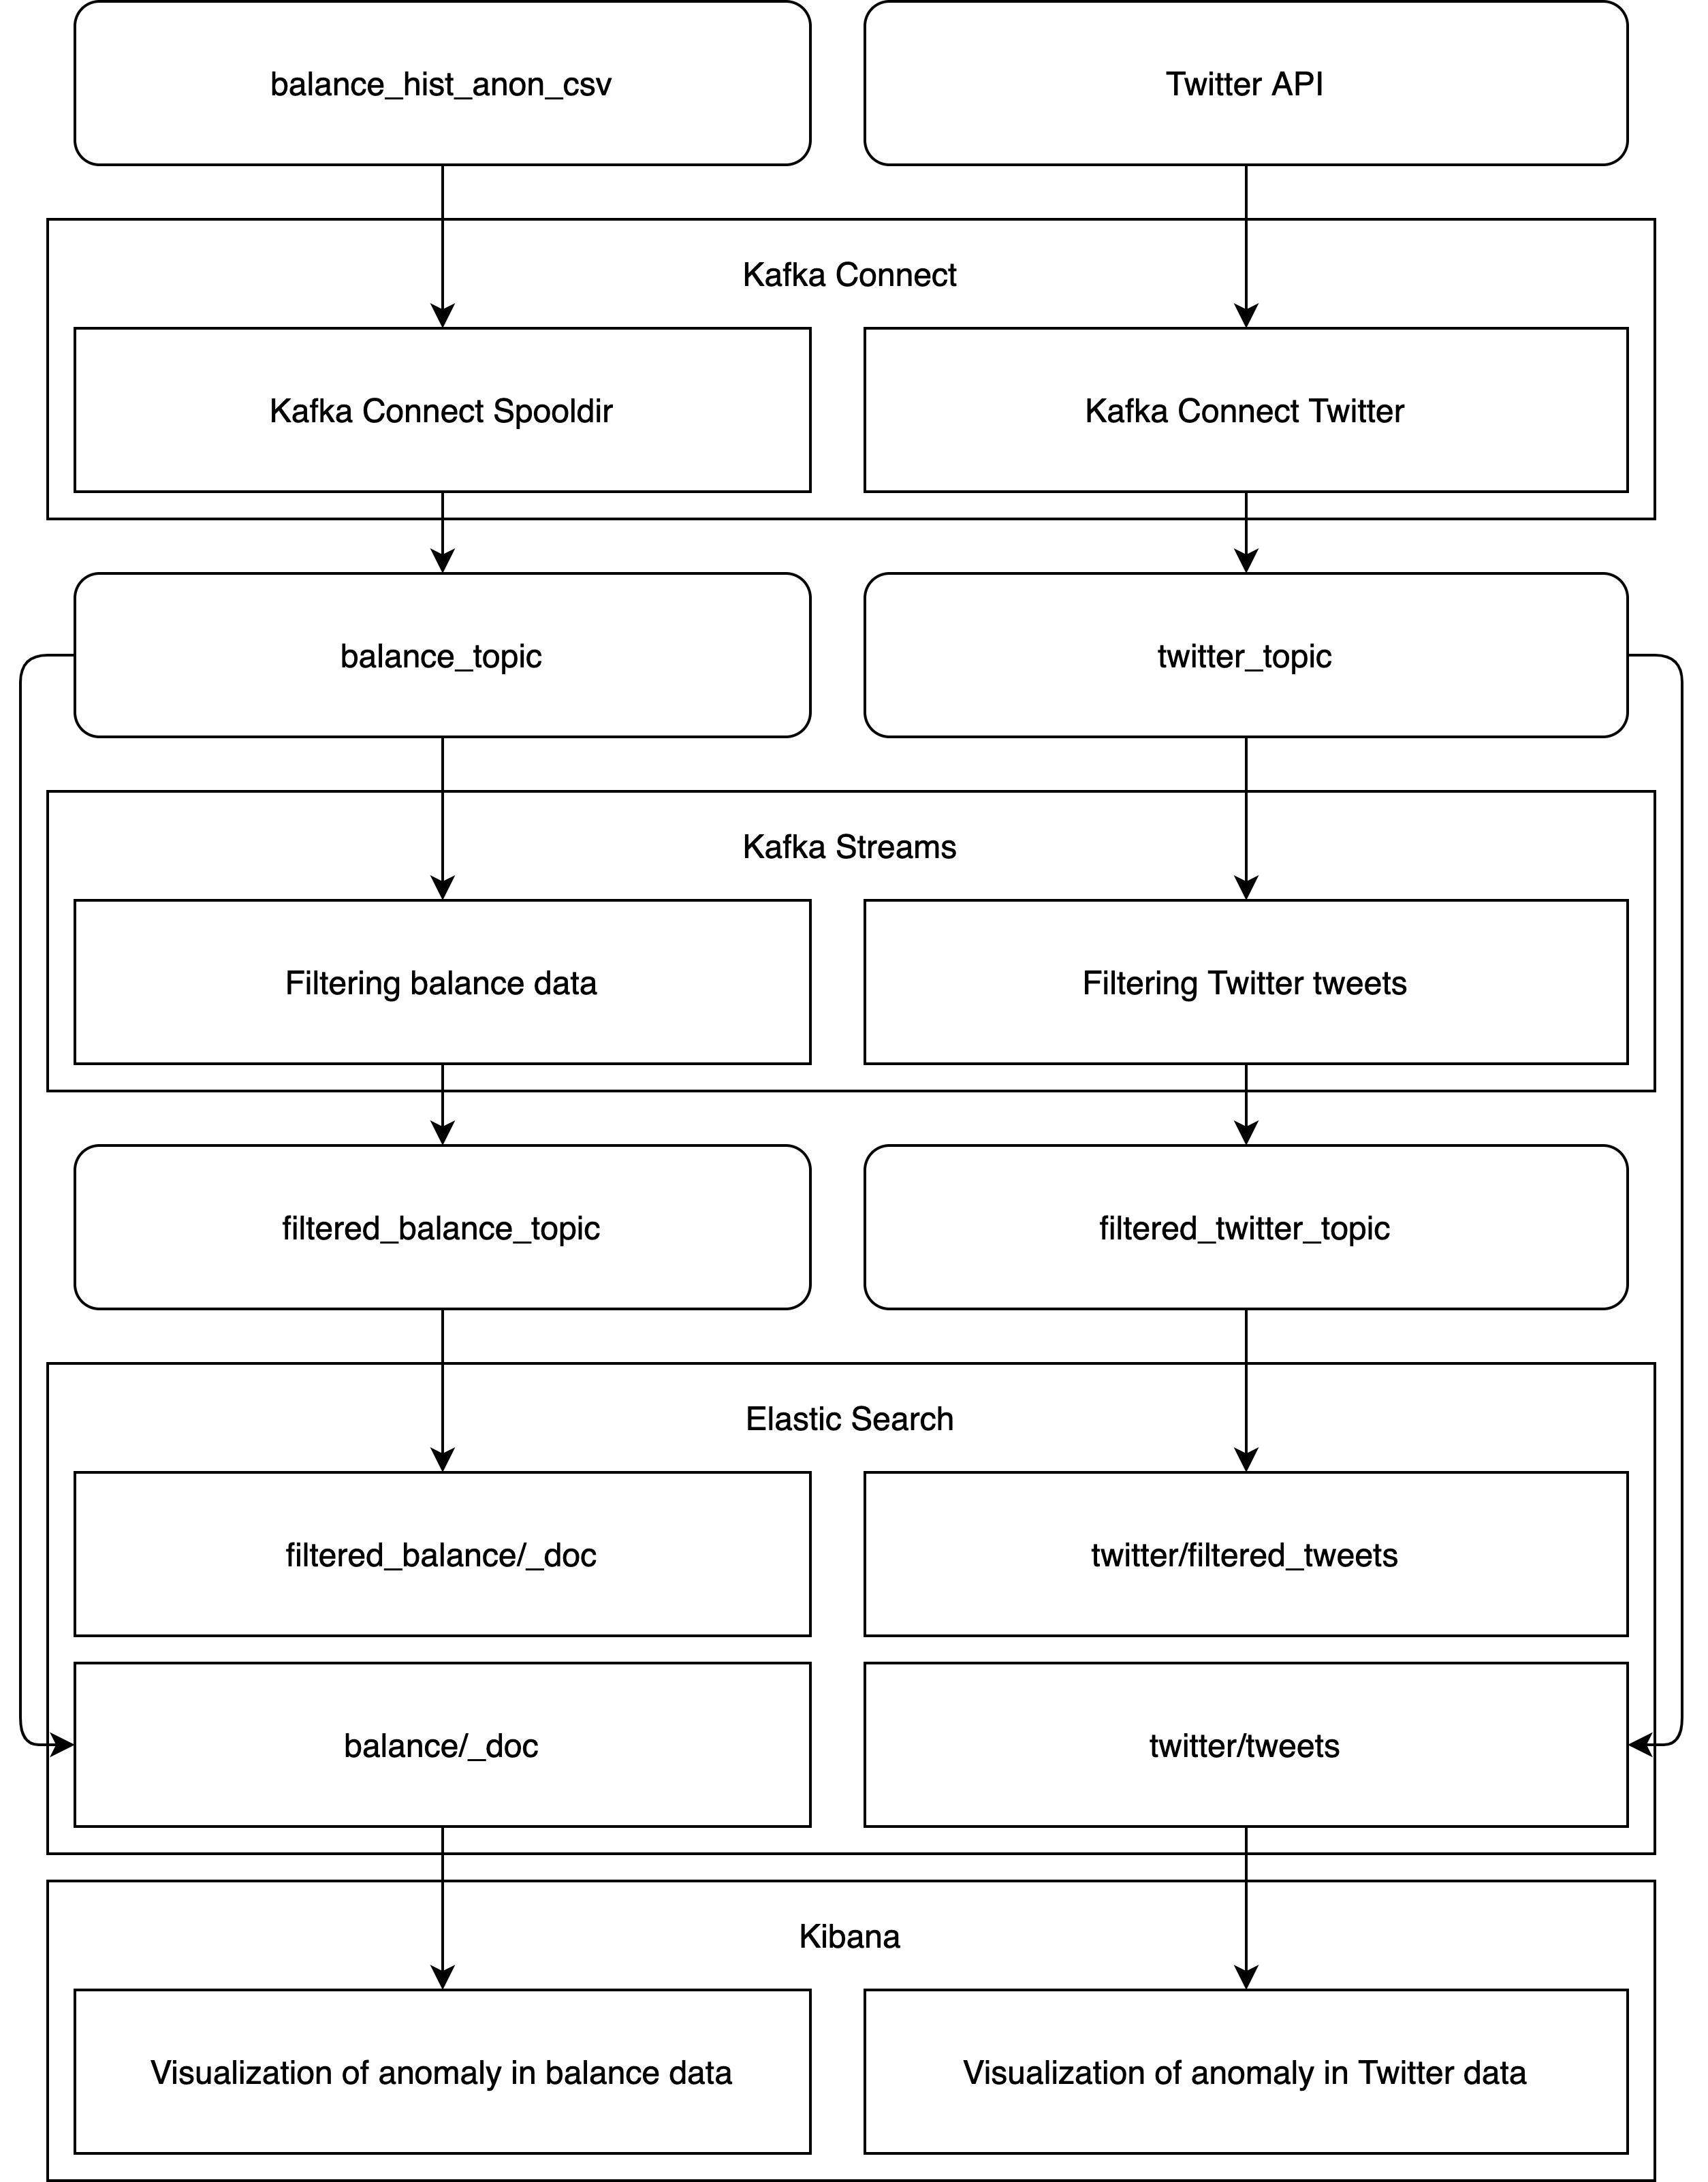
\includegraphics[scale=0.115]{architecture.png}
\caption{System architecture}
\label{fig:universe}
\end{figure}

\newpage
\subsection{Jupyter Notebook}
\subsubsection{Modifying balance data}

Jupyter Notebook was used to understand balance data and rename first column to 'id'. For debugging purposes, it saves part of data (for example, first 10000 rows).

\subsubsection{Modifying exchange rates data}

Initially 'eurofxref-hist.csv' contains exchange rates for 42 currencies from 04.01.1999 till 09.12.2020. According to balance data, only exchange rates for 10 currencies from 02.01.2017 till 09.12.2020 is used. It is important to note that this data set does not contain exchange rates RSD (Serbian dinar).

\subsubsection{Kafka Producer to read csv data}

KafkaProducer.ipynb has the python code to load data from 'balance.csv' to a Kafka topic. Each row is read as a json object using the underlying schema. This was implemented as a first use case to explore use of python for loading data. We then moved on to one of the more sophisticated methods, i.e., Kafka Connect using SpoolDir.

\subsection{Kafka Connect}

\subsubsection{Why Apache Kafka?}

We have decided to use Apache Kafka, because according to Shree et al.(2017), it is "fast, scalable, distributed stream processing platform and fault tolerant messaging system." It is designed for low latency and high throughput\cite{shree}.

\subsubsection{The connector}
Kafka Connect connector called Spool Dir was used to read 'balance.csv' into the stream 'balance\_topic'. It reads CSV file and converts into JSON format according to the given schema. JSON data is sent to 'balance\_topic'. Batch size is 1000 per batch.

\subsection{Kafka Streams}

According to Bejeck (2018), "Kafka Streams is a library that allows you to perform per-event processing of records". Data is processed as it is available.

\subsubsection{Merging balance data with exchange rates data}

Exchange rates data is read from 'exchange.csv' into HashMap. It is used to update balance data from 'balance\_topic'. For example, when exchange rate is 1 EUR=1.1 USD and account balance 1100 USD is replaced by 1000 EUR.

\begin{figure}[h!]
\centering
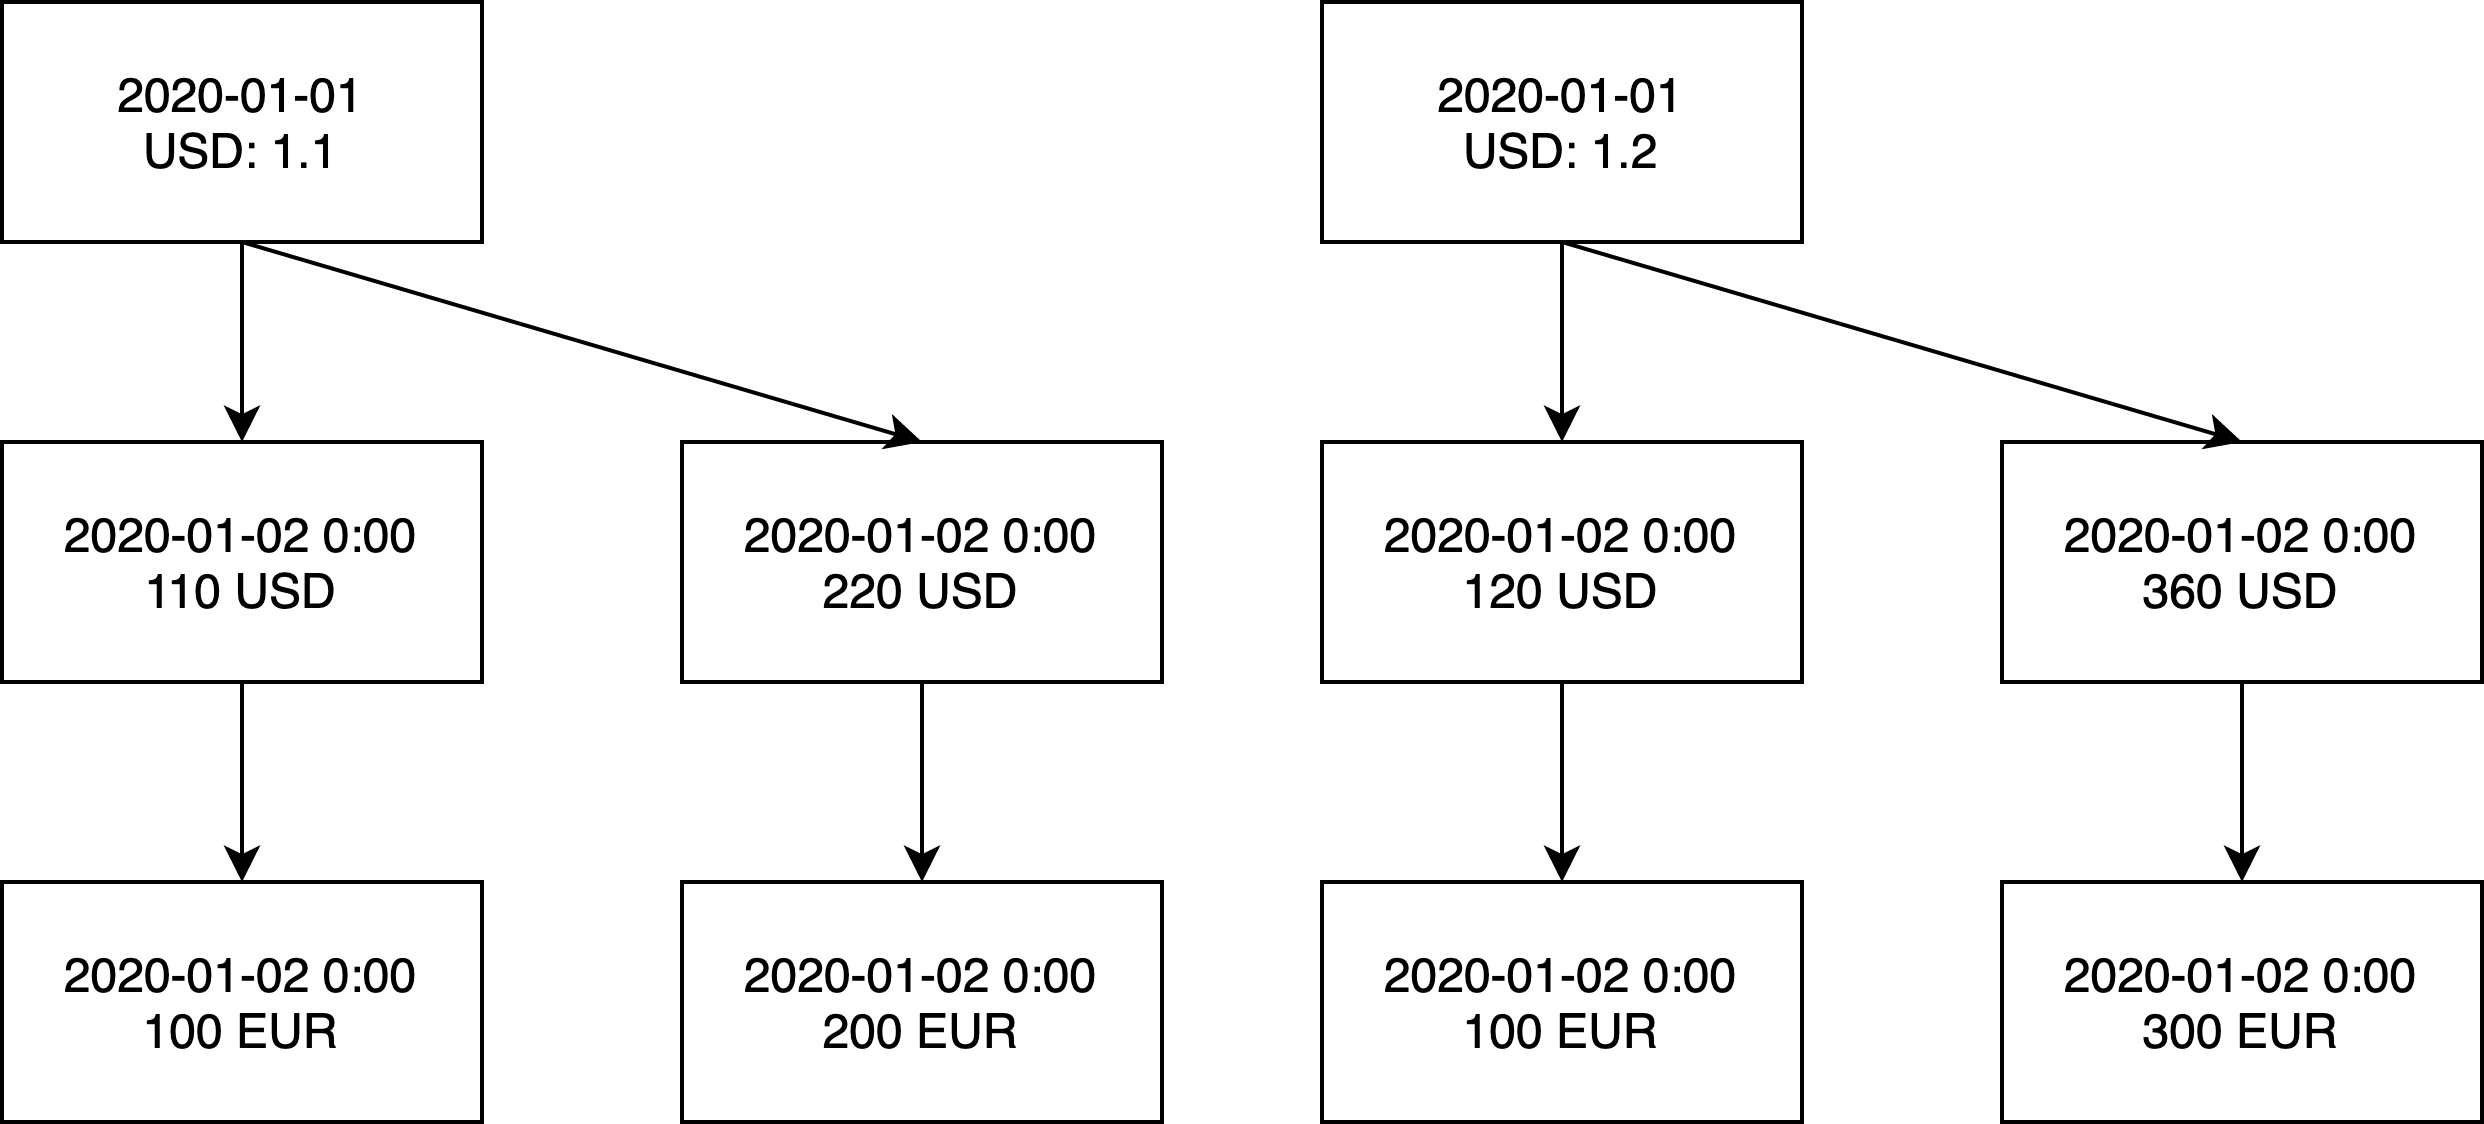
\includegraphics[width=\textwidth]{rates.PNG}
\caption{Merging balance data with exchange rates data}
\label{fig:ExchangeRateMerge}
\end{figure}

\subsubsection{Filtering balance data}

First filtering is made on account balance difference. For this purpose, previous balance amount is persisted by account number. When next account balance state is received, difference is calculated and if the difference is more than predefined limit, it is considered as anomalous. For example, previous balance for the account is 5000 EUR and the current balance is 3000 EUR, the difference is 2000 EUR and it is more than 1000 EUR. This is considered as anomalous and sent to 'filtered\_balance\_topic'.

\subsubsection{Z-score based anomaly on a rolling window}

One of the methods used to determine if a new record flowing into the stream is anomalous or not is the z-score based outlier detection. For every new record entering the stream, the z-score of the balance amount compared to the previous 1000 records is determined. For this purpose, a rolling window of 1000 records is maintained, and the mean and the standard deviation of the records in the window is saved for the 'BALANCE\_IN\_EUR' field. 
Z-score for a data-point in a distribution with mean $\mu$ and standard deviation $\sigma$ is given by the formula:
\begin{equation}
    ZS(x) = \frac{x-\mu}{\sigma}
\end{equation}

If the z-score of the new record on the 'BALANCE\_IN\_EUR' field comes out to be more than a threshold value of 3, then the record is marked as potentially anomalous. This is based on the assumption that the transactions follow a normal or a Gaussian distribution and the records that have a absolute z-score of 3 or more implies that it is more than 3 standard deviations away from the mean of the distribution and is likely to be anomalous (In a normal distribution, ~99\% of the records fall within 3$\sigma$ from the mean)

\subsubsection{Additional ways to filter balance data}

We also detect anomalies for every unique customers in the following way: we measure the mean of the previous spendings, and if the unseen data is deviating very strongly from it then we mark it as anomaly. Since data is coming line line by line, the average is recalculated every time when a new data is arriving. There is a predefined threshold for deciding whether we mark the data as anomaly or not. Also we are measuring the differences between the dates, thus we don't allow a transaction after not using the account for one year, or in case of invalid date data.

\subsubsection{Identifying Anomaly}

Original stream data from 'balance.csv' being loaded into a kafka topic named 'balance\_topic' was analysed using multiple stream transformations to identify anomaly. Two new fields, 'ANOMALY' and 'ANOMALY\_TYPE', were added during the transformation to indicate whether the record was anomalous or not, and if yes, then what kind of anomaly was detected. Transformed stream was subsequently loaded to ElasticSearch hosted locally and visualized using Kibana.


\subsection{ElasticSearch and Kibana}

On the consumer side of the pipeline, we chose to use ElasticSearch as the database and Kibana for visualization. ElasticSearch is easily configurable and can overcome issues in real-time data analysis which is otherwise challenging in other NoSQL or relational database services[4]. Kafka consumer module was written to stream the transformed data with information on anomaly to ElasticSearch. Kibana console was used to create, monitor and delete ElasticSearch indices, explore data loaded to ElasticSearch, and create dashboard to visualize the anomaly detection results.

\begin{figure}[h!]
\centering
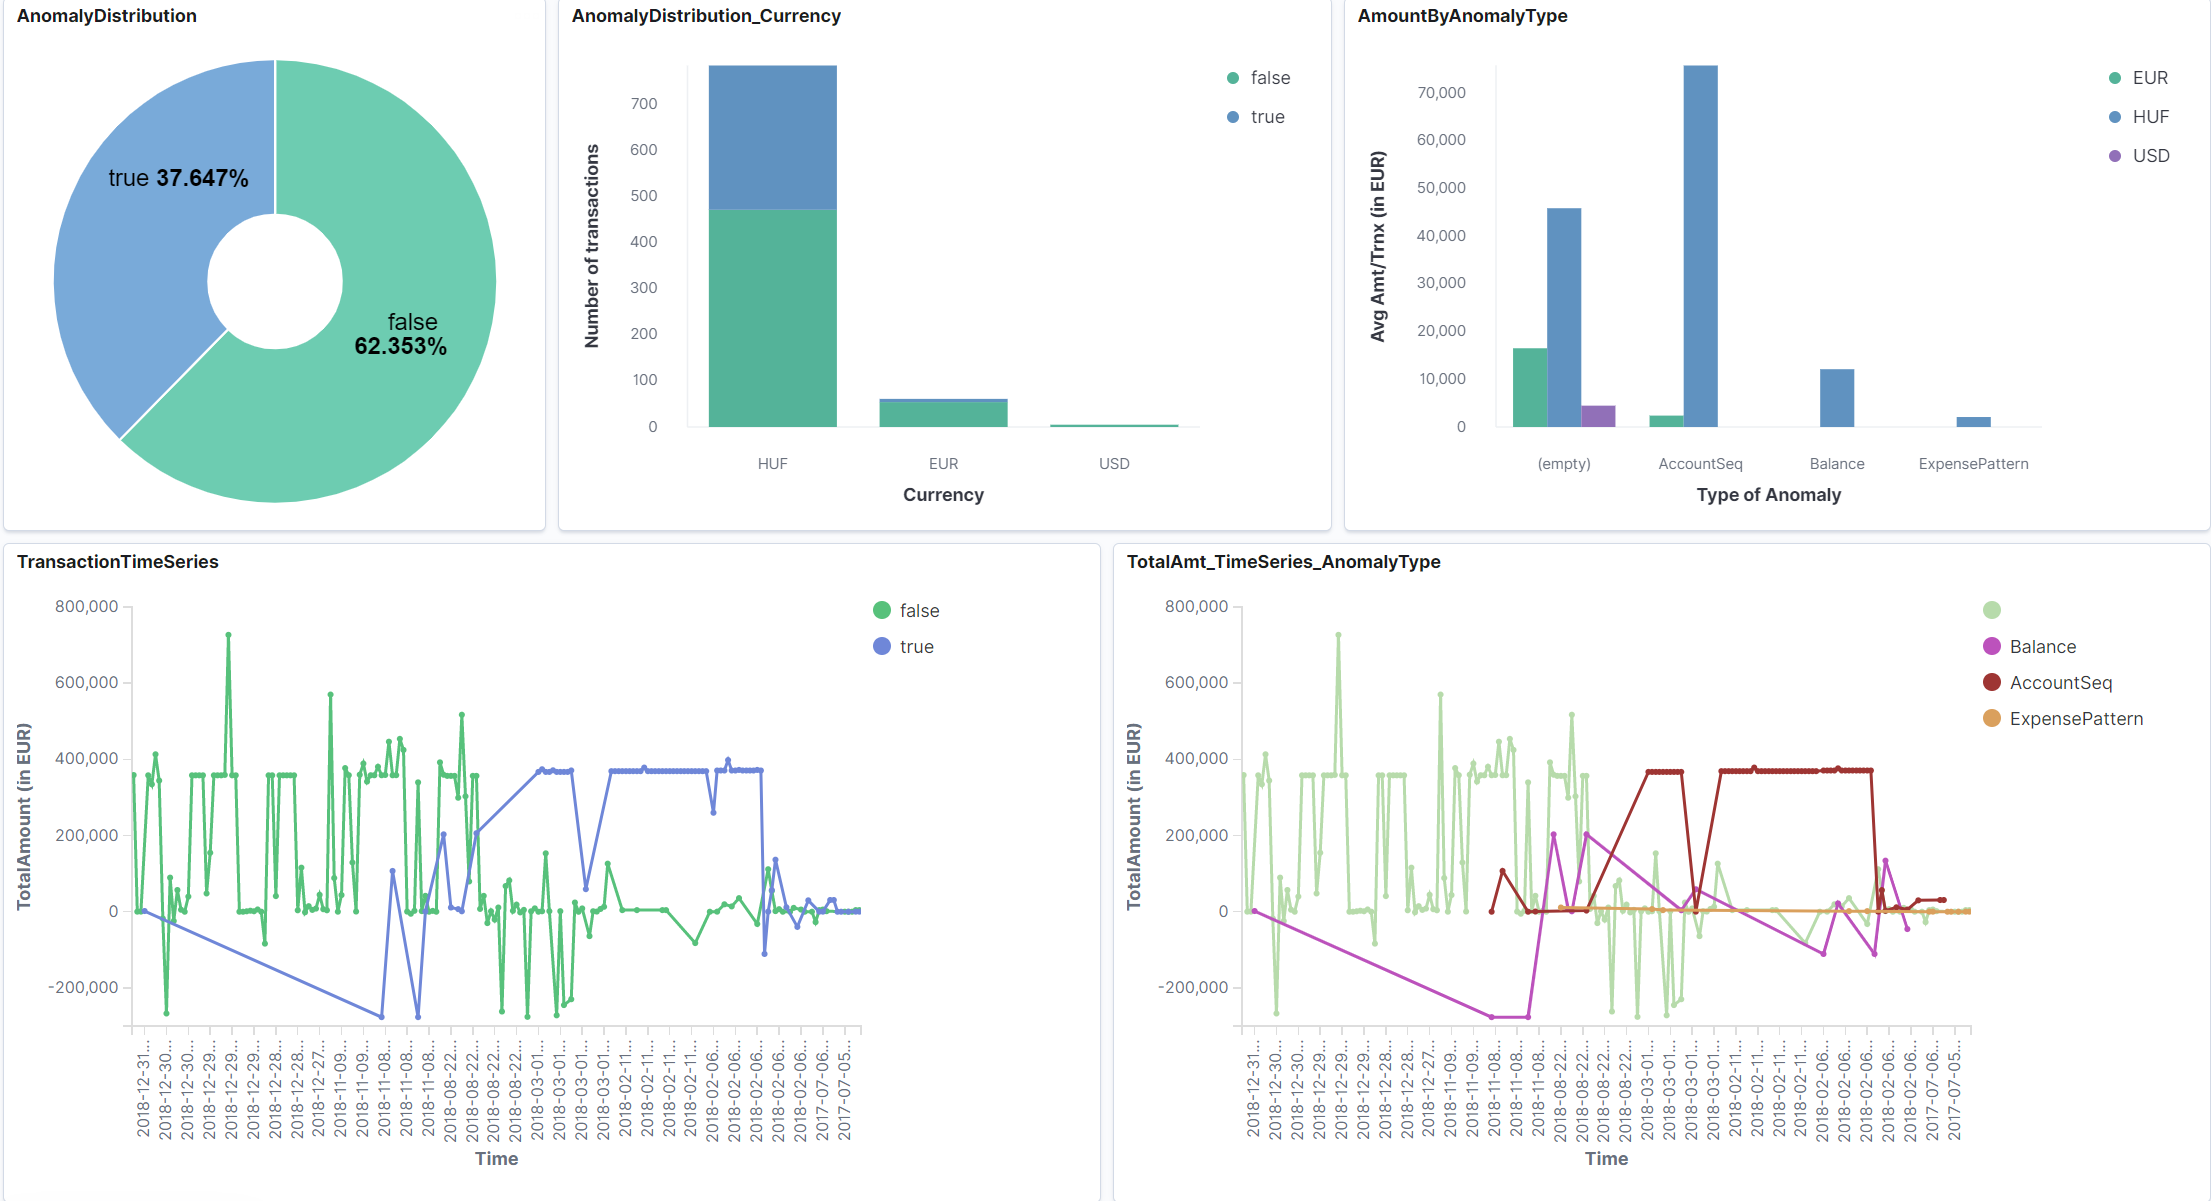
\includegraphics[width=\textwidth]{Dashboard_snapshot.PNG}
\caption{Snapshot of dashboard created in Kibana}
\label{fig:OuptutDashboard}
\end{figure}

\section{Execution Steps}
The overall pipeline of the project can be summarized in following steps:
\begin{itemize}
    \item Start the Zookeeper server (usually in port 2181)
    \item Start the Kafka server (usually in port 9092)
    \item create a kafka topic to load the csv data using the kafka-topics command. Choose number of partitions and replication factor accordingly. (In our project, replication-factor was set to 1 since Kafka server was hosted locally with a single broker)
    \item use Kafka Connect to load csv file to the kafka topic created earlier using the SpoolDir connector
    \item created another kafka topic to load the transformed and processed stream
    \item execute the kafka stream processing code that includes the exchange rate information and performs transformations to identify anomalous data records
    \item start ElasticSearch server (usually on port 9200)
    \item start Kibana server (usually on port 5601)
    \item create index using Kibana console to load the data to be visualized
    \item execute kafka consumer module to load processed stream to ElasticSearch within the created index
    \item Open the kibana dashboard and set the refresh rate to required frequency and monitor the output. 
\end{itemize}

\section{Experiments}

\subsection{Merging 2 streams}

It was tried to merge the balance data and currency exchange data streams into one using Kafka Streams. However, during the implementation of this idea, several problems were faced. For example, the way how to synchronize daily exchange rates with balance data on the given date was not found. Primitive merging of two streams caused the following problem: the balance data is received before exchange rate data for specific day and balance data could not be updated. For this reason, exchange rate data was read directly from file without creating stream.

\subsection{Twitter API}

It was tried to use Twitter tweets feed to help find anomalies on balance data. For example, tweets with keyword "HUF/USD", "HUF/EUR", "Economy of Hungary". However, the meaningful use case of tweets feeds was not found and it was decided to not to use them.

\subsection{Kafka Producer in python}

As a parallel method to read data from csv file to kafka topic, a kafka producer module was written in Python using the kafka-python package. Since a more sophisticated approach to load csv file with underlying schema definition using Kafka connect was figured out, this other approached

\subsection{Remote ElasticSearch server}

Twitter all tweets and filtered tweets are stored in remote ElasticSearch server called Bonsai. It was found out that it is convenient way to set up ElasticSearch server in short time. However, according to the project requirements balance data should not be stored in third party storage. Further, only upto 10k records can be loaded to ElasticSearch database hosted in Bonsai under the free version. Due to these limitations, it was decided to use ElasticSearch and Kibana servers hosted locally on our personal computers.

\subsection{Docker containers}

Docker provides lightweight virtualization technology, which can be useful if we just want to run applications in separated environments. We don't need to virtualize a whole OS which could be very resource demanding. We decided to use docker containers for Elasticsearch and Kibana. After configuring the ports, we can use them in a very effective way since we don't need to use online solutions like Bonsai. It can be useful also when lot of people are working on the code, since it is very easy to share environments, and set them up. At the end everyone will have the same environment, which makes development a lot easier.

\begin{figure}[h!]
\centering
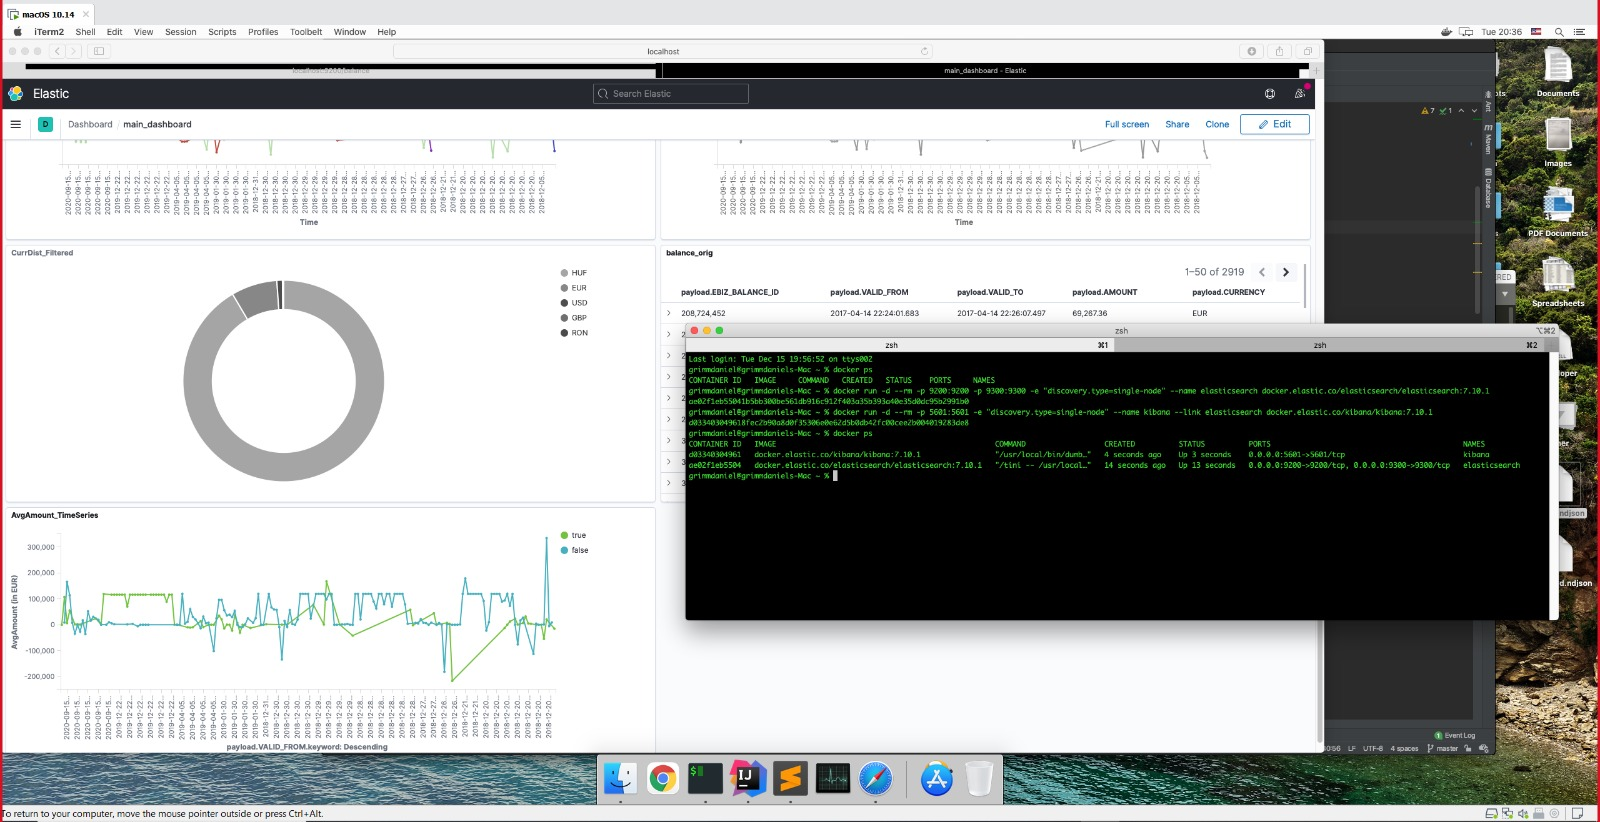
\includegraphics[width=\textwidth]{Docker_snapshot.jpg}
\caption{Workflow with Docker containers}
\label{fig:OuptutDashboard}
\end{figure}

%\section{References}

\newpage
\begin{thebibliography}{9}

\bibitem{ecb}
European Central Bank. (2020). Euro Foreign Exchange Reference Rates. \url{www.ecb.europa.eu/stats/eurofxref/eurofxref-hist.zip?53a6f7cba144c040b7a2a4a8242d1431}.

\bibitem{shree}
Shree, R., Choudhury, T., Gupta, S. and Kumar, P., (2017). KAFKA: The modern platform for data management and analysis in big data domain. 2017 2nd International Conference on Telecommunication and Networks (TEL-NET), 1. \url{https://ieeexplore.ieee.org/abstract/document/8343593/}

\bibitem{Bejeck}
Bejeck, B. (2018). Kafka Streams in Action: Real-time apps and microservices with the Kafka Streams API (1st ed.). Manning Publications.

\bibitem{Shah}
Shah, N., Willick, D. & Mago, V. (2018). A framework for social media data analytics using Elasticsearch and Kibana. Wireless Netw. \url{https://doi.org/10.1007/s11276-018-01896-2}

\bibitem{shafi}
Shafi (2018). Docker, Elasticsearch and Kibana (part 1) \url{https://medium.com/@s\_tokhi/docker-elasticsearch-and-kibana-c76808ea3ab8}

\bibitem{rahasak}
Rahasak, Λ. (2020). Kafka and Zookeeper with Docker. https://medium.com/rahasak/kafka-and-zookeeper-with-docker-65cff2c2c34f

\end{thebibliography}

\end{document}